
\twocolumn[\begin{@twocolumnfalse}
{\begin{minipage}{7.75in}\begin{center}\begin{minipage}{5in}

\begin{abstract}
\noindent{}This chapter provides an overview 
of certain data structures associated 
with biomedical research, as well 
as summarizing some of the 
technological and clinical 
contexts wherein data modeled 
via these corresponding structures 
is acquired.  We will motivate 
this discussion by reviewing basic 
principles of personalized medicine 
and patient-centered care in the Covid-19 context.  
Later chapters will pursue a more abstract, systematic, 
or holistic account of these 
(and similar) data structures, 
data types, and data profiles construed as 
formal artifacts essential to 
digital information spaces, computational 
environments, and software design 
patterns.  In this first chapter, 
however, our goals are more 
empirically-minded, trying to 
convey a sense of the biomedical 
data landscape by describing 
several important varieties of 
biomedical information, as a 
precursor to more theoretical 
discussions later in the book.
\end{abstract}

\end{minipage}\end{center}\end{minipage}}
\end{@twocolumnfalse}]
\thispagestyle{empty}
\cleardoublepage{}



\addcontentsline{toc}{section}{Chapter 2: Data Structures Associated with Biomedical Research}

\addtocounter{page}{-1}


\hoctitle{Chapter 2: Data Structures Associated with Biomedical Research}
\vspace{1pt}


%\p{}

\section{Introduction}


\p{\:\+Covid-19, cancer, and Cardiac Care are among
the most significant health-care challenges
of our time. \> The devastation wrought by
the SARS-CoV-2 pandemic, both in terms of
lives lost and global economic impact, is
well-known. \> Cancer and Heart Disease are
if anything even deadlier. \> Covid-19 erupted into
the world's attention in early 2020; cancer and
Heart Disease have not had their own
single crisis moment,
but they have been at the forefront of scientific
attention for decades, spurring treatment
innovations and scientific breakthroughs.\;\<
}

\p{\:\+Covid-19 is a coronavirus very similar to the
SARS strain that caused many deaths in 2004;
like all viruses in their class, these pathogens
use spike proteins to invade the human host's
respiratory system, spreading to the lungs and
sometimes affecting cardiac and neurological
functioning as well. \> Many cases of Covid-19
are mild or asymptomatic, but for still-obscure
reasons about 16\% of infected individuals
require hospitalization, including a 3-4\% mortality
rate. \> All this is widely known, reported in everyday
newspapers and web sites as well as scientific journals.\;\<
}

\p{\:\+But how \i{do} we know these details? \> Different facets of
Covid-19 \mdash{} its genetics, proteins, biomechanics,
epidemiology, mutations, treatment options, and so forth
\mdash{} are the province of different biomedical
specializations. \> The complete picture of
Covid-19 therefore has to be assembled from many different
lines of research. \> Much information about the
virus was acquired soon after the start of the pandemic,
and the development of effective vaccines has progressed
at a torrid pace. \> Such accelerated results,
unprecedented in medical history, reflect well on the
current state of biomedical knowledge and competence
of the practitioners of biomedical sciences worldwide.
\> While Covid-19 data is imperfect, and much remains
mysterious about this disease, scientists' opinions should
generally be taken seriously (and not politicized or
obfuscated for ideological reasons).\;\<
}

\p{\:\+Nevertheless, there is no harm in trying to get a
deeper understanding of \i{how} Covid-19 science
has progressed so quickly. \> For anyone approaching
Covid-19 from an angle outside of biology or
health care proper \mdash{} be that public policy,
ethics, economics, sociology, or technology
(and so on) \mdash{} trying to understand
the chain of scientific reasoning is not a matter
of pre-empting scientific expertise, but
of trying to comprehend the Covid-19 crisis
in a well-informed manner. \> What were the crucial
insights gleaned from SARS-CoV-2 genomics, morphology,
and biomechanics, as well as from contact tracing
and clinical observations, which allowed a
useful picture of Covid-19 to fit together in
just a few months in 2020? \> How does the
cryptic numeric data driving models of SARS-CoV-2's
genes, proteins, or anatomy get translated
to intuitive pictures of the virus as an active biological
agent, with its specific infectious tendencies
and deadly effects on human hosts?\;\<
}

\p{\:\+To be sure, a thorough recount of the scientific history
unfolding through the Covid-19 pandemic would
require a much longer book than this one.
\> We will not, in other words, directly attempt
to excavate scientists' detective work
in early 2020 in the manner we just hypothesized,
however much that is a story that inevitably
\i{will} get told sometime after the pandemic
has receded. \> But we \i{can} touch on one
very specific field within this overarching
trajectory, namely the role of
computer software and the kind of data
which forms a first step toward comprehensive
models of diseases (and their treatments and interventions).
\> This applies, of course, to cancer/oncology and
Cardiac Care as much as to Covid-19.\;\<
}


\p{This first chapter will focus on certain specific 
data types which emerge from contemporary 
research methods and clinical/diagnostic data-acquisition 
modalities (including specialized equipment which 
itself represents a form of technological breakthrough, 
such as high-throughput gene sequencing).  We will 
also consider how the goals of \q{personalized} medicine 
have motivated the search for data-integration 
methods working on these data structures emerging 
from new biomedical technologies.  Our goal is 
to look at certain concrete data structures 
--- their computational profiles, 
representation formats, and scientific 
foundations --- as a precursor to 
later chapters' more theoretical discussions 
of data types as software artifacts.}

\p{\q{Biomedical Technology} is an umbrella term 
which encompasses many more specific topics 
and subdisciplines.  Different investigative 
modalities --- from genomics to proteomics to 
bioimaging (to name just a few) --- tend to 
have their own technological ecosystem.  Scientists 
who concentrate on specific fields within the biomedical 
umbrella therefore become familiar with technology 
(meaning both computer software and lab equipment) 
which is used in their area of study.  There is less 
impetus for an overarching expertise that would 
encompass biomedical software in a more holistic 
sense, which potentially yields lacunae in 
biomedical software engineering.  There is, in short, 
relatively little research into design patterns 
which might be generally applicable to biomedical software 
as a whole.}

\p{At the same time, with the rise of Precision Medicine, Patient-Centered Care, 
and systems-biologic paradigms which integrate multiple 
anatomical and biochemical scales (from molecules to cells 
to tissue and organ systems), biomedical research has 
become interdisciplinary to an unprecedented degree.  One 
consequence of this (generally positive) trend is that 
software ecosystems and computational paradigms targeted 
at specific subdisciplines prove to be suboptimally 
fragmented.  Cross-disciplinary research implies the need 
to connect hitherto isolated software ecosystems together.}

\p{Our goal in this chapter is to make these issues tangible 
by identifying several specific biomedical subdisciplines 
and the data structures which they tend to generate.  
These are the kinds of heterogeneous data models that 
need to be integrated in order to provide a computational 
foundation for multi-disciplinary biomedical research.  
We are not attempting to develop a comprehensive 
list of bioinformatic data-types, but merely to 
describe certain data models which are especially 
important and recurring in contemporary science.  
Hopefully these concrete examples can help oriented 
our analyses when we transition to more abstract 
discussions about data types, data models, and 
software-development paradigms.}

\p{This chapter will consider \q{personalized medicine}  
in the context of Covid-19 (later chapters will 
address personalized medicine in its more 
traditional settings, particularly immuno-therapies 
as promising approaches to cancer care), so 
we adopt Covid-19 as a lens for examining the 
origin and clinical significance of data structures 
emerging from technologies such as Next-Generation 
Sequencing and bioimage analysis via Computer Vision.  
However, data structures characteristic of these 
technologies are, for the most part, widely used 
in clinical and diagnostic practice; they are not 
specific to Covid-19 (here we will not emphasize 
research which is more narrowly targeted at 
SARS-CoV-2, such as biophysical analyses of 
the virus's proteins, or epidemiological studies 
of the pandemic's origins).}

\p{Gauging public sentiment, it has been suggested that  
patients during the Covid-19 pandemic are increasingly reluctant to participate in 
conventional trials where they run the risk being assigned 
to a control group where they might lose the opportunity 
to receive life-saving treatment.\footnote{See, for instance, 
\cite{IanDWolfe}, or 
\bhref{https://www.pharmacytoday.org/drugs/drugs-2020-04-22-story4}. 
Also \cite{JCBlader} is an interesting discussion about the merits of 
double-blind trials (and in particular the idea 
of \q{unblinding} follow-up studies), albeit 
well before Covid.}  
In this context Shrestha \textit{et al.}'s approach 
may be justified as more consistent with patients' 
wishes for their own care, wishes that 
should be taken seriously in patient-centered contexts.}


\p{Shrestha \textit{et al.} represents only one publication, 
but their philosophy of trial design perhaps portends a 
paradigm-shift away from individual, controlled studies 
and toward nonrandomized, concurrent trials.  
In lieu of single investigations comparing an 
experimental group with a control group, 
concurrent trials allow the results of 
different studies to be compared against 
one another; each trial serves as a \textit{de facto} 
control \visavis{} each concurrent trial.  Integrative 
data-modeling tools thereby steers  
patients into different trials based on personalized data 
packages (which may include immunological, cardiovascular, 
neurological and other general medical-history 
data) obtained for each patient prior to their involvement 
in a trial, and likewise made available 
for subsequent analysis.}


\section{Personalized Medicine in the Context of Covid-19}
\p{Within just a few months after Covid-19 became a global pandemic, 
doctors and researchers were developing and experimenting with a 
diverse range of treatments and remedies against SARS-CoV-2.  
The treatments which were in some sense 
tested or adopted include Monoclonal Antibodies, 
remdesivir, dexamethasone and other steroids, anti-inflamatory drugs
(such as tocilizumab and sarilumab), 
convalescent plasma, baricitinib (a rheumatoid arthritis 
drug for which Covid-19 is an off-label use), and 
anti-malarial drugs (specifically chloroquine and 
hydroxychloroquine).\footnote{\i{See} \bhref{https://www.mayoclinic.org/diseases-conditions/coronavirus/expert-answers/coronavirus-drugs/faq-20485627}.}
These treatments, that is to say, were either approved (albeit 
provisionally or \q{for emergency use}) by the United States \FDA{} and other 
government agencies, pending clinical trials, 
or reported anecdotally to be helpful in combating Covid-19.  In either 
case they were relatively widely adopted in clinical settings.  
More rigorous attempts to validate claims of any treatments' 
effectiveness, however, have proven inconclusive (at least 
as of mid-2021) --- certainly 
no pharmaceutical or clinical intervention has demonstrated success 
rates comparable to the first wave of vaccines that were approved 
toward the end of 2020.  In short, every well-studied Covid-19 intervention 
(other than vaccination) appears to be successful in some patients and 
not others.  These mixed results generate questions of their 
own --- what are the biologic mechanisms that 
cause different treatments to play out differently 
in distinct patient populations?}

\p{Of course, it is possible that associations between 
treatments and outcomes --- at least in the SARS-CoV-2 context 
--- is driven mostly by random chance, or that treatments 
are correlated to, rather than causative of, outcomes.  
The Covid-19 mortality rate among hospitalized patients 
appears on average to be less than 25\% (even though  
over four million people worldwide have died from 
the pandemic, as of summer 2021).  Accordingly, many people 
even with serious cases of Covid-19 will recover just 
via statistical distribution.  While it 
is possible that treatments received in 
hospitals account for some of the recovery rate ---  
the mortality rate amongst hospitalized patients has diminished 
over time, which implies that hospitals have become more 
skilled in caring for Covid-19 patients and that treatment 
plans have become more refined --- many 
patients hospitalized for the disease might well have recovered 
anyhow (even without additional pharmaceutical or clinical 
interventions).  
Given this interpretive uncertainty, it has been difficult 
for researchers to definitively show that particular 
treatments do in fact improve recipients' chances of 
recovering from Covid-19.  Nevertheless, both observational evidence and 
clinical trials suggest that a number of Covid-19 treatments 
do have some positive benefits, even if not for all patients.}

\p{This situation then leads to the question of why 
particular treatments benefit some patients more than 
others.  Such considerations are of scientific interest, 
of course --- clarifying how drugs or other interventions 
interact with the SARS-CoV-2 virus enhances our knowledge 
about its infectious mechanisms and the progression of 
Covid-19 --- but more immediately it is of clinical 
interest, because doctors need guidelines on 
when to administer which treatment(s) to which individual 
patients.  Since no Covid-19 remedy (apart from vaccination) clearly 
outperforms others under most circumstances, scientists have 
attempted to study Covid-19 treatments with the goal of 
giving doctors more detailed information to work 
with when making these sorts of clinical decisions.  The overarching 
project of a significant subset of Covid-19 research, 
in short, has been to establish criteria allowing doctors 
to predict which treatments are most likely to succeed 
for individual patients, given details of their 
immunological profile and prior medical history.}

\p{In this sense the goals of Covid-19 research overlap with 
methodologies that have been established in the context 
of other research areas --- notably cancer and AIDS --- 
under the general rubric of \q{Precision Medicine.}  
As a field of research, Precision Medicine is focused on 
the correlation between patient-specific biomedical details 
and the likelihood that particular interventions will have 
positive effects for particular patients.  In contrast to 
conventional clinical trials, which consider patient-specific details 
only at a rather coarse level --- merely observing obvious 
data-points such as age, gender, and ethnicity --- precision-medicine 
research attempts to curate a much more detailed picture of 
patients' medical and sociodemographic profiles, either as 
part of formal trials or as observational details in a clinical 
setting.  Ideally, Precision Medicine is motivated by the 
goal of analyzing patient-profile-to-outcomes correlations 
not only retroactively (detecting statistical patterns in 
prior outcomes) but also prognostically.  In effect, once a 
particular sort of treatment has been identified as 
especially favorable for patients with certain characteristics, 
it is reasonable to project that future patients with similar 
characteristics should be given similar treatments.  
This intuitive and obvious point, however, masks empirical 
and practical difficulties --- in particular, it is not 
obvious how to quantify the notion that current patients 
are \q{similar} to prior ones.  Indeed, one of the 
provisional results of precision-medicine research thus far 
has been to highlight how statistically significant points of 
resemblance between patient profiles do not necessarily line 
up with how we \textit{intuitively} group patients together by 
visible factors such as age, race, or gender.}

\p{In sum, Precision Medicine has been guided by the thesis that 
compiling detailed patient-centered information can advance 
clinical medicine by identifying which treatment options 
are more likely to succeed for individual patients.  In the 
context of Covid-19, both the diversity of legitimate 
clinical interventions and the failure of any one 
treatment to show unambiguous success for a broad spectrum of 
patients point to the potential usefulness of patient-centered 
approaches.  If doctors have detailed information about 
Covid-19 patients' immunological profiles and 
clinical history they can --- at least in theory --- make 
informed decisions about which treatment options have a 
higher probability of success.  Such predictions would 
not be a matter of guesswork; instead, statistical analysis 
of Covid-19 cases in the past, preferably backed by 
Machine Learning, would detect correlations between 
patient data and recommended treatments.  In effect, the 
spectrum of possible Covid-19 interventions (antibodies, 
steroids, convalescent plasma, and so forth) serves as a 
natural classifier, grouping patients into clusters based 
on pre-treatment profiles indicating that one or another 
Covid-19 intervention has, with some probability, a good 
chance of helping the patient.  Researchers have therefore 
been seeking empirical clues for how to classify patients 
into categories based on recommended treatment plans.}

\p{We will examine in this chapter how the 
goals of Precision Medicine have spurred scientists to propose 
more sophisticated data-integration 
and data management tools in the context of clinical trials 
and biomedical laboratory investigations.  Aside from 
opening new avenues for empirical research, the \textit{goals} 
of Precision Medicine have spurred new ways of 
thinking about the computational ecosystem which supports 
biomedical research and clinical practice. 
}

\subsection{Precision Medicine as a Catalyst for Biomedical Data Sharing}

\p{Precision medicine is based on the scientific realization that the effectiveness of a certain clinical intervention --- for instance, 
immunotherapy as a cancer treatment --- is dependent on factors that 
vary significantly between and among patients.  In the case of immunotherapy for cancer, assessing 
the likelihood of favorable outcomes requires genetic, serological, and oncological tests which need to be 
administered prior to the commencement of treatment.  
Therefore, analysis of precision-medicine outcomes requires detailed 
immunoprofiling --- building immunological profiles of each patient before 
(and perhaps during/after) the immunotherapy regimen --- alongside 
an evaluation of how well the patient responds 
to the treatment, with the best outcome being 
cancer remission or non-progression.}

\p{The contemporary emergence of Precision  
Medicine is driven, in part, by advances in diagnostic 
equipment which enable immunological profiles to be 
much more fine-grained than in previous decades.  This 
level of patient-profiling detail enables granular three-way analysis 
involving (1) patients' immunology; (2) treatment 
regimens; and (3) clinical outcomes.  This three-way approach 
has the goal of 
identifying signals in immunological profiles that indicate 
which therapeutic interventions are most likely to engender 
favorable outcomes.  As with any statistical analysis, 
predictive accuracy increases in proportion to the amount 
of data available.  As such, further refinement of 
precision medicine  
depends in part on data aggregation: pooling a number of 
observational studies where patients' immunological profiles 
are described, in detail, alongside reports on treatment plans 
and patient outcomes.}

\p{Within the scientific research community, organizations such as the 
Society for Immunotherapy of Cancer (\SITC{}) and 
the Parker Institute for Cancer Immunotherapy (\PICI{}) 
have developed 
programs and tools to share immunotherapy research 
data, which join older (but less cutting-edge) 
projects, such as Cancer Commons or the \RSNA{} 
(Radiological Society of North America) Image Share program.  
In the Covid-19 population we are similarly 
presented with multidimensional patient data.  
Such information traverses 
molecular testing to identify the virus's genetic material 
or the unique markers of the pathogen itself; antigen testing 
(albeit less accurate) to identify specific proteins found on 
the outer surface of the virus; mapping the genomes of SARS-CoV-2 
to learn how it mutates; analyzing blood samples for the presence/absence 
of antibodies in response to a prior SARS-CoV-2 infection; using 
high-dimensional flow cytometry to perform taxonomic breakdown of 
patients into distinct immunotypes related to disease severity and 
clinical parameters; profiling patients' immunological state prior 
to the start of treatment and quantifying patients' immunological 
response once treatment has begun; calculating plasma viscosity (\PV{}) 
for detection of unusually high levels of fibrinogen --- 
leading to atypical blood clots (that are refractory to 
standard anticoagulant therapy); monitoring 
cognitive, neurological, or cardiovascular  
symptoms in \q{long haulers}; and so forth.}

\p{One area where data-integration is significant for Covid-19 research 
is that of protein biomechanics.  For instance,
\cite{QiongqiongAngelaZhou} identifies  
64 different proteins which are therapeutically 
relevant to Covid-19.  Each of these proteins can be connected to molecular data, 
bioassay information and, in many cases, to clinical 
trials that test therapies where the specific protein acts as a 
target for inhibiting SARS-CoV-2.  
In combination, aggregating all of this information yields a
heterogeneous (but interconnected) 
data space, characterized 
by data derived from multiple scientific disciplines and multiple 
laboratory methods.}


%\section{Overcoming Impediments to Data-Sharing Initiatives in Precision Medicine}
%\subsection{Data-Sharing Solutions for Immunoprofiling/Immunotherapy and Covid-19}

\p{Because biomedical diagnostic and investigative 
laboratories need to use highly specialized software, 
raw laboratory data is often excluded from data-sharing initiatives.  
Instead, the information which is shared between 
hospitals or research centers tends to be a simplified 
overview --- adhering to standards curated by 
groups such as  
\OMOP{} (Observational Medical Outcomes Partnership) 
Common Data Model or \CDISC{} (Clinical Data Interchange Standards Consortium) 
--- skews more toward succinct summaries of diagnoses, treatments, and/or 
outcomes.  Limitations in sharing more granular 
diagnostic or prognostic data have been identified as obstacles diminishing 
the value of data-sharing initiatives.  As one example, in a 
paper discussing research  
into the sequencing of immunoglobulin repertoires (Ig-seq), 
\cite{SimonFriedensohn} comments: 

\vspace*{.5em}
\begin{displayquote}
A major challenge when performing Ig-seq is the production
of accurate and high-quality datasets [because] the conversion of
mRNA ... into antibody sequencing libraries relies on a number of 
reagents and amplification steps ... which potentially introduce errors
and bias [that] could alter quantitation of critical 
repertoire features. ... One way to address
this is by implementing synthetic control standards, 
for which the sequence and abundance is known prior to sequencing, thus
providing a means to assess quality and accuracy.
\end{displayquote}
The underlying 
problem in this context is how different laboratories may use 
different techniques and protocols to achieve similar diagnostic/investigative 
goals (\i{see also} \cite{LauraLopezSantibanezJacome}, 
\cite{MarksDeane}, \cite{MartijnMVanDuijn}, \cite{YanlingWu}, 
etc.).  Consequently, when data is merged from multiple hospitals, it is likely that 
the raw data derives from different labs, which can lead to situations where  
protocol variations across each site can introduce errors
and bias that contaminate the aggregate data-sharing results.  
(We should note that Ig-seq and related \q{repertoire sequencing} 
is quite relevant to coronavirus immunology because 
these techniques help quantify patients' immune response 
to infection, which is consequential both for 
explaining the differences between mild and severe 
cases and observing the effectiveness of interventions 
such as vaccinations or antibody treatments; 
\i{see} \cite{KatjaFink}, \cite{AnastasiaAMinervina}, 
\cite{ChristophSchultheiss}, \cite{NataliaTFreund}, \cite{JacobDGalson}, 
\cite{AleksandraMWalczak}, \cite{CheMaiChang}, 
 \cite{SupriyaRavichandran}, \cite{RishiRGoel}, 
etc.)}

\p{In the context of Covid-19, Shrestha \textit{et al.} 
\cite{GentleSunderShrestha} argue 
for \q{precision-guided studies} to be prioritized \q{[r]ather 
than conducting trials using the conventional trial designs and 
poor patient selection} (page 1).  To accomplish this, the authors 
recommend \q{large multicenter trials} which incorporate 
\q{predictive enrichment strategies ... to 
identify and thus target specific phenotypes [patient-profile 
characteristics], potentially raising the possibility of positive 
trial outcomes.}  The underlying problem identified by Shrestha \textit{et al.} 
is acquiring sufficiently large trial cohorts 
in contexts where trials are to be targeted at 
fine-grained patient populations with specific pre-treatment 
immunological profiles.  This problem can be 
ameliorated by merging prospective patients from 
multiple institutions, such that concurrent trials spanning 
multiple health-care settings can be launched as part 
of a comprehensive approach to comparing treatment options.  
Such large multicenter trials  
can produce \q{large cohorts of patients in a shorter 
time period} while also steering patients toward 
more favorable treatment courses.}

\p{In short, Shrestha \textit{et al.} 
explicitly challenge the conventional wisdom which 
assigns \q{gold standard} status only to \textit{randomized} 
trials, arguing that the benefits of larger trial sizes 
and quicker trial initiations outweigh whatever 
statistical value is compromised by earmarking 
patients into trials based on educated guesses as 
to favorable outcomes (which is warranted by 
patient-care ethics in any case).  The authors also  
argue for a \q{robust data 
infrastructure} which would combine the efforts of clinicians, researchers, 
and data scientists.  In effect, aggressive data-curation would 
substitute for double-blind trial design as a means 
of ensuring the scientific value of trial outcomes.}

\subsection{Software Alignment for Covid Phylogeny Studies}% across Multiple Populations}
\p{The study of SARS-CoV-2 mutations is another area  
where software alignment can prove to be important.   
Analyses in 2020 suggested that variations in the 
viral strain causing Covid-19 symptoms may be partly 
responsible for divergent immunological responses to 
the virus across the patient 
population \cite{OsmanShabir}.  If one 
patient 
responds 
either less favorably or more favorably than the average patient-response 
to a 
given treatment, clinicians need to assess whether this 
difference can be explained solely by the patient's 
prior immunological profile or whether the patient has 
been exposed to a genetically divergent viral strain.
In 2021, of course, predictions about SARS-CoV-2 mutations 
came to pass, with at least four variants appearing to be 
sufficiently dangerous (by virtue of their infectiousness 
and/or lessened effectiveness of treatments or vaccines) 
to undo progress which has been made against Covid-19 
in many parts of the world.}

\p{Comprehensive models of Covid-19 variants require a 
combination of genetic, proteomic, anatomic, and 
epidemiological information, because mutations can 
only take hold if they modify the virus's morphology 
and/or infectiousness in ways that are conducive to 
that strain replicating.  The \b{delta} strain, 
for example, which (as of mid-2021) has been the 
most wide-spread mutation \cite{LizSzabo}, 
carries a genetic variation (designated 
as \q{\b{D614G}}) 
which results in a denser 
array of spike proteins, thereby reinforcing 
the biomechanic pathway which the virus uses 
to infect the host's respiratory system 
\cite{BetteKorber}, \cite{AnwarMohammad}, 
\cite{UtsavPandey}, \cite{LizhouZhang}, 
\cite{DonaldJBenton}, \cite{ErikVolz}, 
\cite{ShiZhao}, etc.}

\p{Modeling SARS-CoV-2 evolution across the globe is a 
massive project.  There have been over 200 million Covid-19 cases 
worldwide (as of mid-2021), in virtually every nation on earth, so a 
complete phylogenetic picture of SARS-CoV-2 in 
humans would need to pool data from many different 
healthcare systems.  Yet, even technically 
detailed analysis of the phylogeny of SARS-CoV-2, such as that 
conducted by Dearlove \textit{et al.} (as 
reported at the end of 2020) 
only considered 27,977 patients (about 0.1\% of 
global cases), with almost half from the 
United Kingdom \cite{BethanyDearlove}.  
Hence, achieving something resembling a holistic picture of 
SARS-CoV-2 mutations and how they might affect clinical 
treatments, would require many parallel studies analogous 
to that of Dearlove \textit{et al.}.}

\p{This then raises questions of study alignment: calculating 
viral phylogeny requires making technical decisions about how genetic 
sequences should be acquired and analyzed, decisions which 
may vary among research teamss.  
For example, Dearlove \textit{et al.} describe several computational 
steps which they had performed 
both to normalize each SARS-CoV-2 genome sequence in their 
data set for cross-comparison and to run predictive 
simulations (used to estimate whether divergence between 
sequence-pairs are the result of localized, random mutations or, 
conversely, an indication that SARS-CoV-2 is evolving into 
further distinct strains).    
Clustering SARS-CoV-2 genomes into variants --- that 
is, identifying which mutations are random and which 
appear to be propagating to subsequent viral generations 
--- involves making computational and biological 
assumptions, such as how to statistically 
marshal genomic data so as to quantify the prevalence of a 
mutation, and how to estimate whether a particular mutation confers 
an adaptive benefit to the viral agent (e.g., an 
ability to elude antibodies targeting structural proteins).}

\p{Given that modeling viral phylogeny requires 
certain computational assumptions and biological 
guesswork, data from multiple studies can only be 
reliably integrated if there is some degree of 
alignment across their methodology.  As such, 
research teams should document their protocols 
in a manner that permits assessment as to whether 
protocol differences might compromise the 
resulting data.  One way to achieve this is to 
model the protocol itself as a data type in a 
general-purpose programming 
language (such as \Cpp{}, for sake of argument).  For each study, such as 
Dearlove \textit{et al.} cited above, there would then 
be a \Cpp{} object encapsulating details of 
the researchers' protocols and computational workflows.  
Protocol-alignment would in this context 
be one part of a common framework to quantify the 
epidemiological significance of SARS-CoV-2 mutations.}

\p{In short, a holistic 
global picture of SARS-CoV-2 must represent 
SARS-CoV-2 mutations which have been deemed 
phylogenically and/or clinically significant (i.e., having 
potential either to influence the overall evolution of 
Covid-19 and/or to have some bearing on clinical treatments), 
and must \textit{also} represent divergent SARS-CoV-2 strains 
carrying those mutations.   
These data-points 
are then be the basis of further details such as: 
when did a given strain and/or mutation first appear?  Is 
the strain/mutation geographically localized?  What is the 
proportion of different strains/mutations in a geographic 
area?  Is there evidence that different strains/mutations 
affect a patient's immunological response to Covid-19 and/or 
the effectiveness of vaccines, antibody regimens, steroids, 
or other clinical interventions?  How can genetic mutations within 
the SARS-CoV-2 virus be correlated with structures in the spike 
proteins encoded by the viral genes?  This last question points 
to the importance of integrating genomic data with \ThreeD{} molecular 
models (\textit{see} \cite{WingerCaspari}, \cite{SandipanChakraborty}, 
\cite{IvanMercurio}, \cite{AliFAlsulami}, \cite{SumanPokhrel}, 
\cite{VictorPadillaSanchez}, \cite{FedaaAli}, for example).  
Whereas data structures modeling the viral genome 
are composed of nucleotides --- and, at a higher scale, Open Read 
Frames (\ORF{}s) --- data structures describing the biophysics of 
glycoproteins involve protein architecture and chemical 
bonds \cite{LiangweiDuan}, \cite{AnshumaliMittal}, 
\cite{XiuyuanOu}, \cite{GiwanSeo}, \cite{HanhTNguyen}, 
etc.  Analyzing how 
\makebox{SARS-CoV-2} genes 
affect the production of glycoproteins, therefore, requires 
annotating and cross-referencing nucleotide/\ORF{} data structures 
with \ThreeD{} molecular models encoded in formats 
such as \MOL{} or Protein Data Bank (\PDB{}) 
\cite{YasunoriWatanabe}, \cite{YongfeiCai}, \cite{AlexandraCWalls}, 
\cite{GennadyMVerkhivker}, \cite{CheolminKim}, etc.}

\p{Object-Oriented models for genomic phylogeny analysis 
have been presented in \cite{JoshuaBSinger} 
(Java) and \cite{GuanghongZuo} (\Cpp{}), although 
these do not provide object models to extend 
from genetic information toward clinical, proteomic, 
or imaging data.  We are not aware of Object-Oriented models 
proposed as representational devices 
for Covid Phylogeny in this more holistic and 
interdisciplinary, but this form of 
software design would be consistent with code 
developed in contexts such as oncology, for 
example the computational simulation of 
tumor growth, which we will discuss in Chapter 4.  
Covid-Phylogeny Object Models 
could serve as a nexus for merging temporal and 
geographical data concerning the epidemiology of \makebox{SARS-CoV-2} 
mutations with genomic data demonstrating  
which mutations are significant, as well as clinical 
data tracking correlations between mutations and treatment outcomes.  
Supporting multi-trial data integration would, therefore, 
also introduce new requirements for clinical trial software, 
which we discuss further next chapter.}

\subsection{Personalized Medicine and Immuno-Profiling}
\p{While some of the data related to immunological profiles 
may be sociodemographic or part of a patient's medical history (fitting 
nicely within conventional Clinical Research 
Network models), contemporary 
immunoprofiling is powered by 
highly specialized diagnostic equipment and methods --- 
which require special-purpose file formats and software.  
For instance, one dimension of immunological profiling is \q{immune repertoire};
the more robust a person's repertoire, the wider variety of antibodies they can produce to fight off pathogens.  Immune repertoire is often measured by studying genetic diversity in B-cells; in recent years, 
this has been done using \q{Next Generation Sequencing} (\NGS{}), which produces files in formats 
such as \FASTQ{}.  Another dimension of immunological profiling is quantifying the proportions of different sorts of blood cells in a patient's blood sample, which is typically done via Flow Cytometry or Mass Cytometry, yielding \FCS{} (Flow Cytometry Standard) files.  The immunological evaluations which are the goal of these methods are sometimes called Cell-Type Classification or \q{Automated Cell-type Discovery and Classification} 
(\ACDC{}).}

\p{As outlined in the below table (Figure~\ref{fig:tabl}), immunological profiles draw on a diversity of data formats and lab/data-acquisition modalities (this table is not intended to be a complete list of criteria or file formats, but rather to indicate the range of diagnostic technologies and data formats which are relevant to immunoprofiling).  This table hopefully indicates how immuno-oncology data sharing 
is inherently more complex when compared to data-sharing 
initiatives which focus primarily on 
clinical outcomes --- such as  
\OMOP{}, \CDISC{}, or the Patient-Centered Outcomes Research Network 
(\PCORnet{}).}


\begin{figure*}
\caption{Table Outlining Several Data Formats and the Contexts where they are Acquired}
{\large
\vspace{1.5em}
\begin{tabular}{ l | r | c }
\underline{Immunological Profile Dimension} \hspace{.5em} & \underline{Lab/Clinical Method} \hspace{.5em}   & \underline{File Format} \\
Sociodemographic                & \hspace{.3em} Scan Patient Records \hspace{.3em} & CSV, SQL \\
Medical History                 & \hspace{.3em} Scan Patient Records \hspace{.3em} & CDISC, OMOP, PCOR \\
Immune Repertoire               & \hspace{.3em} NGS \hspace{.3em}                 & FASTA, FASTQ \\
Cell Type Classification        & \hspace{.3em} Flow/Mass Cytometry \hspace{.3em} & FCS \\
Immune/Tumor Microenvironment         & \hspace{.3em} Confocal Microscopy \hspace{.3em} & \hspace{.4em} DICOM, OME-TIFF, CoCo

\end{tabular} 
\vspace{1.5em}
}
\label{fig:tabl}
\end{figure*}




\p{Formats such as the  \OMOP{} Common Data Model (\CDM{}), the \PCORnet{} \CDM{}, 
or the \CDISC{} specifications promote data sharing primarily through 
\SQL{}-style tables, where 
data analysis and extraction can be achieved via conventional 
\SQL{} queries.  The situation is very different, however, when 
the data that must be exchanged derives from specialized hardware 
and software, which demands special-purpose file formats, parsers, 
and query engines.  This problem-space is accentuated 
when preparing multi-site sharing that can span dozens of 
hospitals, research centers, and/or laboratories.  
Problems of cross-institutional data integration 
will be analyzed further next chapter.}

\p{Prior to that discussion, the following section 
will examine in detail the file formats and data structures 
which were briefly mentioned thus far in this chapter.  
Our goal in this discussion is to document the 
kinds of data which are endemic to different branches 
of biomedical research.  A separate analysis --- one 
which to some extent depends on first describing the data 
formats involved --- concerns how to fuse multiple 
data formats into a common overarching format, such as a 
\q{Common Data Model of Everything.}  One recurring 
theme we will encounter in the subsequent discussion is the 
goal of merging certain data profiles into others 
(e.g., \FCS{} into \DICOM{}), or else adopting 
common interchange formats (such as \XML{}) in lieu of 
domain-specific binary formats which demand 
special-purpose parsers.  We will examine both the strengths 
and weaknesses of proposals for adopting common formats 
rather than idiosyncratic \q{legacy} formats that 
are tied to particular laboratory methodologies for 
historical reasons.  However, our main purpose in the 
current discussion is to establish basic facts about 
data formats in current use.  Later chapters will 
analyze problems connected to the integration of these 
formats into common data models.} 

\p{Note also that the following inventory of biomedical 
data formats is by no means exclusive.  In particular, we 
have largely neglected antigen tests, biochemical assays, 
and many other lab techniques which rely on chemical 
reactions to obtain lab/diagnostic findings.  Our discussion 
here is oriented more toward methodologies which require 
relatively complex intermediate computational processing 
to arrive at clinically useful findings.}





\section{A Review of Certain Commonly-Used Biomedical Data Formats}

\p{Because a major focus of this book is the goal 
of \textit{integrating} disparate data structures into a common 
format, it is an important preliminary step to examine the 
data formats which need integration to begin with.  For reasons 
explained above, this list is by no means exhaustive or 
comprehensive; nevertheless, the data profiles considered 
here constitute a representative spectrum of structures 
which are important to contemporary bioinformatics.}

\p{Note in addition that some of these data formats are 
demonstrated in computer code which we have prepared to 
accompany this book.  The authors have republished and/or modified 
open-source libraries used to parse data in the formats discussed 
in this section, and we provide examples to demonstrate how 
these file formats are used in real-world contexts.  For each 
format there is an accompanying code project (associated with a 
\Qt{} \textbf{.pro} file) which can be opened in the 
\Qt{} Creator \IDE{} and compiled.  The resulting executable will 
load a sample file and use parsers endemic to the file format 
being discussed.  The details of each format may accordingly 
be studied by looking at the computer code for parsing the 
files and/or by running the demo programs through a debugger.  
More information about how to use these demonstration 
code libraries for pedagogical purposes is provided along 
with the code samples themselves.}

\subsection{DICOM (Digital Imaging and Communications in Medicine)}

\p{The \DICOM{} format is closely associated with 
the \PACS{} (Picture Archiving and Communications System) standard 
for sharing biomedical images; both formats together constitute the 
\textit{de facto} standard for bioimaging in clinical and 
diagnostic settings.  A \PACS{} workstation is guaranteed to 
have certain capabilities with respect to the diversity of image-formats 
the software can receive and process from outside sources.  This level 
of standardization is important because biomedical images are 
commonly shared amongst disparate institutions; for example, 
radiographic images generated in a hospital may be sent to a 
laboratory for diagnostic processing.  The \DICOM{} and \PACS{} 
standards guarantee that recipients of images will be able to 
view and share them properly, assuming that the images are 
provided in certain canonical formats and with certain basic 
metadata (it is worth noting that, in the absence of metadata, 
it may be impossible for software to display images because of ambiguities 
in color depth, color format, image dimensions, and other 
details which determine how binary image data is translated to 
visual pixel renderings).  These standards eliminate the sorts of 
delays which might otherwise be caused when a lab, for example, is 
unable to view images sent by a hospital or doctor's office.}

\p{Although the primary purpose of \DICOM{} is to facilitate image 
transfer, a close second in importance is properly associating 
the images with relevant clinical metadata.  Images are 
typically grouped into series, which are associated with 
specific patients and specific diagnostic goals (often 
diagnostic codes described via fixed vocabularies, such as 
the \q{Radiographic Lexicon,} also known as RadLex).  In the 
Covid-19 context, for example, lung x-rays may be requested 
to support a SARS-CoV-2 diagnosis and/or to test how far the 
disease has progressed into the patient's lungs.  At a minimum, 
them, all images generated for that diagnostic purpose need 
to be grouped together in the current clinical 
context (specifically that this image-series results from a 
possible Covid-19 diagnosis and has a specific clinical/diagnostic 
purpose) and associated with a specific patient (usually identified by 
some sort of anonymizing code).  This residual non-image information 
needs to be tracked via metadata, typically represented within 
\DICOM{} \q{headers.}}

\p{Given that \DICOM{} thereby serves as a forum for exchanging 
general patient info, not only images themselves, the \DICOM{} 
standard was designed to be flexible and extensible.  This has led 
the scope of \DICOM{} to expand of the years, encompassing a 
greater diversity of graphics data (\ThreeD{} images, audio, video, 
ultrasound, etc.) and also non-image content (such recommended treatment 
plans, image annotations, or diagnostic comments).  The \DICOM{} 
system is oriented to enabling these scope-extensions without 
breaking backward compatibility with older \DICOM{} standards.}  

\p{All \DICOM{} data is associated with classificatory \q{tags,} which 
indicate the type of information asserted by a given data-point 
and how it is encoded.  Each tag is assigned a \q{group number} 
and an \q{element number}; this two-layer organization allows 
tags to be grouped together which serve a similar purpose or 
derive from a similar clinical or diagnostic context (the 
pairing of group numbers and element numbers may be 
roughly compared to \XML{} namespaces and element names).  
Different \DICOM{} group numbers are used to group 
tags into those specific to, for example, image data  
(e.g. image dimensions and color model), series/study 
data (date, patient \ID{}, accession number, etc.), patient-specific 
information (birth date, gender, native language, and many other 
data-points), and numerous additional group numbers specific 
to different kinds of images (or other graphics content, such as 
video) which may be present in a \DICOM{} series.  
Officially recognized \DICOM{} groups are each assigned 
\textit{even} group numbers.  The \textit{odd} \DICOM{} 
group numbers can be used for non-standard \DICOM{} extensions, 
but \DICOM{} clients are not required to parse or recognize 
tags with odd group numbers.  In effect, organizations are 
free to use odd \DICOM{} groups to encode any information 
they believe is relevant, but there is no guarantee that 
third parties accessing their data will be able to interpret 
these non-standard codes.}

\p{Another important detail pertinent to the \DICOM{} data model 
is that \DICOM{} files freely combine binary 
and textual data.  Most data in \DICOM{} tags such as those 
just described is textual data, encoding character-based 
details such as a patient's name or date of birth.  Of course, 
\DICOM{} also has to encode binary image data as well.}

\p{In this context, note that many \q{file formats} are 
actually \textit{zipped} files which are unpacked into 
\textit{folders} behind-the-scenes (so that they are actually 
\q{folder formats}).\footnote{For example, \textbf{e-book} files 
are merely zipped files encoding entire book directories, 
which generally include different files for individual chapters, 
images and other non-textual content, and metadata in formats 
such as \XML{}.}  Programmers familiar with formats based 
on zipped folders might instinctively feel that the natural 
way to fuse textual and binary content is to create 
folders wherein the two sorts of content are spread across 
different individual files.  For example, an \XML{} file could 
encode textual data such as that present in most \DICOM{} 
tag-groups, whereas a series of image files could store 
the individual series images.}

\p{However, the \DICOM{} 
standard embraces a much different architecture, where 
\DICOM{} tags introduce data streams that may be either 
textual or binary; the tag itself (in fields immediately 
following the group and element numbers) asserts the number 
of bytes need to encode information belonging to that tag, 
and those bytes may be interpreted either as character-streams 
or as binary sequences holding (in particular) image data.    
Whereas file formats that expand to unzipped folders are 
\q{file-based} (in that, once the unzip step is completed, 
information is spread across multiple files), \DICOM{} is 
\q{stream-based} --- all \DICOM{} data, from an identifier 
tag which requires only one or two bytes to be encoded to 
a video asset that may run into megabytes of size, 
is inserted into a sequence of tagged byte-streams which 
collectively span a \DICOM{} file.\footnote{As an aside, 
\sDICOM{} tag-sequences can be nested in other tags, so 
technically \sDICOM{} files are hierarchical by analogy 
to \sXML{} or \sJSON{}; however, this hierarchical 
structure is much less common in the \sDICOM{} context 
than in other encoding schemes.  It is reasonable to 
consider the \sDICOM{} format as first and foremost a 
string of sibling tags rather than as a hierarchical 
document structure, for most purposes.}}

\p{The mixture of binary and textual data in \DICOM{} tags 
--- together with idiosyncratic features such as 
numeric group/element tag identifiers rather than character-based 
entity/field names --- sets \DICOM{} apart from most 
serialization formats, which makes it difficult to contemplate 
re-encoding \DICOM{} data in other systems, such as \XML{}.  As a 
result, \XML{} processing algorithms or Semantic Web query formats 
cannot be readily applied to \DICOM{} data; instead, any application 
wanting to query or examine \DICOM{} data streams needs to use 
\DICOM{}-specific code libraries, such as \DCMTK{} (this library 
is reproduced in the code accompanying the present book).  
\lDICOM{}'s opacity to modern query languages has sometimes been a 
source of frustration for programmers, and has led to the 
development of proposals such as \q{Semantic \DICOM{}} which involve 
extracting different sorts of data from \DICOM{} series and 
warehousing this extracted information in databases that are 
amenable to analytic techniques which are not \DICOM{}-specific.  
In so-called \q{Semantic} \DICOM{}, textual header data 
is placed in \NoSQL{} databases of various sorts whereas 
image data is marshaled into individual files, or stashed in an 
image database.  The rationale for this \q{deconstruction} of 
\DICOM{} data is both to analyze \DICOM{} data using non-\DICOM{}-specific 
algorithms and to merge \DICOM{} information with data having 
other profiles.  We will examine Semantic \DICOM{} proposals 
in greater detail in a later chapter.}

\subsection{Next Generation Sequencing and other Genomics Formats}
\p{At the core of all genomics data is the four \q{letters} 
(\ACTG{}, or Adenine, Cytosine, Guanine, and Thymine) which are the 
building-blocks of \DNA{} and \RNA{} (for \RNA{}, Thymine 
is replaced by Uracil, marked with a letter \U{}).  However, genetic 
data is much more complex than merely strings of letters 
drawn from four choices, because genomics files 
also represent groupings of these elements (and also, 
in some contexts, points of divergence amongst two or more genetic 
sequences).  Genomics data structures differ in how these 
groupings and comparisons are described.}

\p{An early and simple example of a genomics file type 
is \FASTA{} (this name derives from the term \q{FAST-All,} and 
originates in a software program which extended an earlier 
\q{FAST-Protein} application).  The \FASTA}{} format is 
used for encoding amino acid sequences as well as nucleotides, 
so numerous letters may be used in addition to \ACTG{}/\ACUG{}.   
Each letter represents either a single nucleotide or a single 
amino acid, and sequences are represented by strings of the corresponding 
letters.}

\p{The other structuring elements of \FASTA{} files are 
\q{comment lines,} which precede sequence notations and 
provide context explaining the source of the sequences.  While 
in theory the comments are human-readable explanations 
which are not formally part of the \FASTA{} format, in practice 
certain structural norms have been adopted in the construction of 
\FASTA{} comment lines, so that these conventions serve as a 
\textit{de facto} extension to the \FASTA{} standard.  In particular, 
\FASTA{} comments often employ references to databases from which 
sequences are obtained, using the \q{pipe} (i.e., vertical-line) character 
(\textscc{|}, Latin-1 code 124) as a field-delimiter.  A more recent variation 
on \FASTA{}, called \FASTQ{}, supplements this sort of contextual 
information with \q{quality scores} which measure the probability 
that a sequence has been read accurately by the physical 
equipment used for the gene sequencing operations that yielded the 
data being presented.}

\p{Genomics file formats have evolved alongside gene-sequencing 
technology.  Genetics has been revolutionized 
in particular by \q{Next-Generation Sequencing,} 
where many small \DNA{} sequences are extracted in parallel 
and then assembled together with the aid of computer software.  
\lNGS{} has made it cost-effective to perform gene sequencing 
on a much larger scale (e.g., a human genome can be 
extracted in a single day), which has greatly expanded the 
quantity of genomics data available to research, while 
also generating a larger quantity of intermediate data 
(because \NGS{} requires a computational infrastructure to 
derive complete results).}

\p{Both of these trends have 
affected the software ecosystem supporting genomics; 
a window onto this evolution can be gleaned by 
considering new file formats which have emerged to encode 
\NGS{}-related data.  For example, the Sequence Alignment 
Map (\SAM{}) and Variant Call Format (\VCF{}) are employed to notate 
both alignment/commonalities among gene sequences and their 
points of divergence.}

\p{In the case of \VCF{}, data structures 
do not represent nucleotide or amino acid sequences directly, but 
instead notate the variation present in one sequence when 
compared against a reference sequence (such as the transposition, 
deletion, or insertion of individual nucleotides).  The \VCF{} 
format is column-based, where one column marks a position in 
the respective sequences where a variation occurs (i.e., the 
sequences have different letters, or one sequence has no corresponding 
letter at all) and other columns provide contextual information, 
including the type of variation and the origin of the divergent 
sample.  The columns present in a given \VCF{} file are 
labeled by a line preceded by a single \q{pound} character 
(\textscc{\#}, or Latin-1 code 35), immediately before 
the raw data.  Prior to this information are \q{header} 
lines which begin with a double-\textscc{\#} and provide information 
\textit{about} the column fields, including their identification 
codes and data types (such as strings, booleans, or floating-point numbers).}

\p{The \SAM{} format is also primarily column-based, 
with an \q{alignment} section comprised of individual lines 
encoding 11 canonical fields as well as potentially other 
optional fields.  The 11 mandatory fields correspond to 
technical details concerning how alignments between 
distinct sequences are discerned (the number 0 or the asterisk 
character are used to represent missing values).  One of 
these fields, treated as a single integer, is actually the 
binary encoding of a bitset --- in other words, a string 
of boolean values, so the corresponding column actually 
represents a collection of roughly 12 individual true/false
data-points.  Optional fields, after the 11 canonical columns, 
are grouped according to two-character tags, accompanied by 
single-character encodings of types (there are only a few 
recognized types in this context, such as signed integers or 
single-precision floating-point decimals).  In addition to 
alignment data, each \SAM{} file has header lines, marked 
by an initial \q{at} character (\textscc{@}, Latin-1 code 64) 
and a two-letter code indicating the header record type.  
Each header line then has a sequence of tab-delimited fields 
which in turn have their own two-letter identifiers.  Note that 
the vocabulary for fields across the \SAM{} format is fixed 
--- every tag or field descriptor has (only) a two-letter code, 
and the set of codes recognized in each context is defined 
by the \SAM{} standard.}

\p{When notating alignments, \SAM{} identifies a 
\textit{reference} sequence against which other sequences 
may be compared (i.e., aligned).  In this context, 
\SAM{} distinguishes between \textit{padded} and \textit{unpadded} 
reference sequences.  The explanation for this distinction 
derives from the nature of sequence variation --- one way that a 
variant sequence may differ from a reference sequence is in the 
\textit{insertion} of a nucleotide or amino acid in a position where 
no corresponding element exists in the reference sequence.  In 
these situations, the most straightforward way to 
notate the variation is to mark a gap in the 
\textit{reference} sequence (typically via an asterisk).  The 
potential problem with this notation is that it conceptually 
distorts the relation between the reference and the variation 
--- the reference constitutes a basis against which a 
variation (or multiple variations) may be defined, so it 
is counter-intuitive to \textit{modify} the reference-sequence 
in light of how variations diverge from it.  A further complication is 
that modifying the reference propagates to modifying all variant 
sequences which do \textit{not} have an insertion at the relevant 
position.  In any case, some applications call for the use 
of \q{unpadded} reference sequences, which have no modifications 
(forcing insertions to be notated with more complex representations), 
whereas others are facilitated by \q{padding} the reference 
base with gaps where one or another variant possesses an inserted letter.}

\p{The preceding overview of genomic file formats has only 
considered structures that encode raw sequence data and its 
alignments or variants; this discussion has overlooked 
any of the tools or notations which build a coherent narrative 
on the basis of sequencing, such as observing how a genomic 
profile has emerged over time.  For example, data visualization 
tools may be used to study genetic variations --- including 
the mutations which have led to divergent strains of SARS-CoV-2 --- 
by picturing them as trees, where branches separate at the point 
of variation on a specific genomic site.  In 
SARS-CoV-2, for instance, one can model the temporal 
evolution of viral variants via data structures 
identifying when a particular strain emerged, from which 
prior strain, and the genomic site where a 
mutation forms the basis of the variant's specificity.  
These data structures, however, are different 
in form and visualizations than the underlying 
genomic data itself.}

%\vspace{2em}
\subsection{The Flow Cytometry Standard (FCS) File Format}
\p{Flow Cytometry uses a combination of lasers and fluorochromes 
to investigate the properties of blood cells, proteins, and other 
cell-scale entities which may be present in blood samples or 
other tissue samples.  Flow Cytometers are machines which 
reduce blood samples (or other fluid samples) to single-cell 
streams and then probe the samples with laser beams.  Depending 
on the size and shape of the cell (or other particle of interest) 
some light will be diffracted around the cell (this is referred 
to as \q{forward scatter}) while other light will reflect off 
the cell (yielding \q{side scatter}).  The combination of 
forward and side scatter provides information about any one particular 
cell; in general, larger cells produce greater forward scatter, and 
more complex cells (complexity in this context is often referred to 
as \q{granularity,} measuring the geometric intricacy of the surfaces within 
or around cells which would scatter light waves in different directions) 
produce greater side scatter.}

\p{Note that these two dimensions are independent 
in general; cells can be both relatively large and relatively complex, 
so that greater forward scatter does not imply lesser side scatter, 
or vice-versa.  In addition to laser probes, modern-day Flow Cytometry 
machines often use a diverse range of fluorochromes to mark cells 
or materials that may be present inside or on the surface of cells, which 
then emit fluorescent light signals that can be absorbed by detectors 
that are placed parallel to the photodiodes and photomultipliers which measure 
forward/side scatter.  Collectively, the scatter signals and 
fluorochromes are called \q{channels.}  The data produced by modern 
Flow Cytometry instruments may have as many as 12 to 14 channels.  
Computationally, the end result is a data structure which 
is notated as a matrix, where each row corresponds to a single 
cell (referred to in coding as an \q{event}) and each 
column represents one channel.}

\p{The canonical format for representing Flow Cytometry data 
is \FCS{} (Flow Cytometry Standard).  Each \FCS{} file encodes 
the \q{event matrix} (essentially a table marking the 
observations for each cell according to each channel; this 
data has no relation to matrices in the linear-algebraic sense 
except that code libraries designed for matrix arithmetic 
are convenient tools for representing the relatively 
large tables that emerge from \FCS{} data).}

\p{Ultimately, the 
purpose of \FCS{} representation is to cluster events 
(that is, individual cells) into groups and then count the 
relative size of each group, which can give information about 
the sample being analyzed --- for instance, a blood sample 
can be examined to measure the ratio of monocytes to lymphocytes.  
Such classification does not emerge automatically from the 
raw event data; instead, a series of mathematical and geometrical 
transformations is often necessary to transform event matrices 
into scatter-plots where event classification becomes 
visually obvious.  The process of clustering events 
subsequent to these transformations is called \q{gating.}  
As a result, a complete description of \FCS{} analysis 
requires the raw \FCS{} data to be paired with representations 
of transforms which are applied to individual channels 
and with descriptions of gates applied to the resulting two-dimensional 
spaces (each space being a side-by-side comparison of two channels).  
Flow Cytometry data is also presented sometimes as a histogram, 
visualizing individual transformed channels on their own.}

\p{Note that 
this discussion has largely equated cells with events, 
given that historically and in practice the most common 
application of cytometry is to quantify the sorts of 
cells observed in a biological sample; however, cytometry 
can also be used to probe other submicroscopic 
(roughly cellular-scale) 
entities, such as microbes (which may be multi-cellular) 
or extra-cellular vessicles (particles that are released 
from cells).  Flow Cytometry can also indirectly 
examine entities which are too small to generate discrete 
events in the raw data; for instance, side-scatter 
and/or fluorescent channels can be used to quantify 
proteins or biomarkers occurring on the exterior of cells.}

\p{Preliminary to raw event data, \FCS{} files also contain 
\q{headers} which present information about the individual 
channels and about the experimental setup (e.g., the 
make and model of the machine used for the actual cytometry).  
Headers in \FCS{} are preceded by dollar-sign characters 
(\textscc{\$}, or Latin-1 code 36).  Some headers 
provide information about the overall experiment, while 
others are specific to individual channels.  These latter 
header fields have a specific internal structure encoded in the 
tag name: in general they contain the letter 
\textbf{P} (for \q{parameter}), followed by a 
number representing the channel, and then an additional 
letter representing which specific piece of 
information is being presented about that channel.  
For example, the code \textbf{\$P9F} would be 
used as a tag marking a string value representing the 
name of the optical filter applied to the 9th channel.  
The \FCS{} standard also allows for post-processing 
information, such as channel transformations and 
gating, to be recorded in \FCS{} headers fields, 
although such information is often instead presented 
in separate files, with formats such as \GatingML{}.}

%Flow cytometer for measurement of the light scattering of viral and other submicroscopic particles

%Flow cytometry: a flexible tool for biomarker research
%Quantification of proteins by flow cytometry: Quantification of human hepatic transporter P-gp and OATP1B1 using flow cytometry and mass spectrometry


\p{There are a variety of mathematical transforms 
which may be applied to channels prior to gating, 
including various logarithmic transforms, and bi-exponential 
calculations (such as transforms based on hyperbolic 
sines and inverse hyperbolic signs).  Considering an 
overall Flow Cytometry workflow, there are in totality, then, at 
least four different stages of observation/analysis which 
must be recorded: machine setup and overall experimental 
properties (encoded via \FCS{} header data); event matrices 
themselves; transform functions which have been applied 
to various channels; and gating steps, or the geometry 
of regions applied to cross-channel scatter plots that 
classify events based on cell types.}

\p{These different 
kinds of data have generally given rise to several 
different file formats, as well as to proposals to 
unify these formats into an overarching common vocabulary, 
potentially replacing \FCS{} (as we will cite 
specifically in later chapters).  One proposal is to encode 
\FCS{} within \DICOM{}; other suggestions are oriented 
around \XML{}.  The rationale for merging \FCS{} within 
the overall \DICOM{} infrastructure derives in part 
from the conceptual similarities between \q{gating} applied 
to \FCS{} scatter-plots and \q{segmentation} of 
biomedical image data --- although \FCS{} plots 
are not images \textit{per se}, they are akin to bioimages 
in that they are obtained through optical instruments and 
can (with suitable mathematical transformation) take on a visual 
form where clusters of related events (evincing a common cell-type) 
are geometrically circumscribed --- roughly analogous to how discrete 
objects form distinguished regions within photographs.  
These conceptual similarities have yielded calls to 
record \FCS{} data according to annotations and 
terminologies associated with image data, which is the 
subject of the next subsection.}   

\subsection{Image Segmentation, Contours, and Regions of Interest} 

\p{Many image-processing use-cases in biology and medicine 
involve isolating particular \q{foreground} regions from 
within diagnostic or laboratory images (e.g., individual 
cells from within a tissue sample magnified via microscopy; 
tumors within a radiographic image intended to diagnose 
solid-tumor cancer; or patterns of ground-glass opacity 
which suggest the presence of SARS-CoV-2 in lung scans).  
The process of isolating particular regions within 
images is sometimes discussed via the generic term 
\q{segmentation,} although technically segmentation involves a 
complete partition of the image, wherein every point of the 
image is assigned to exactly one segment.  The goal of 
image-analysis is often less about segmenting extraneous 
\q{background} material, but rather demarcating 
\textit{Regions of Interest} which are conceptually more 
important than the rest of the image.}

\p{This overall 
theme applies outside of biology as well; image tagging 
refers to the process of classifying images according to their 
most prominent features or objects.  If a photograph is classified 
as an image of a car, for example, the most important 
\q{Region of Interest} is the area which demarcates the car 
itself, considered as a foreground, from other background 
content (perhaps the street or driveway where 
the car is parked).  Similarly, if a microscopic image reveals 
three blood cells, the Regions of Interest are the cells themselves.}


\p{In contrast to other discussions in this section, our 
examination of image-annotation will not focus on specific 
file formats so much as on how regions of interest may be 
characterized.  To prepare this discussion, it is useful 
to consider a concrete example of how Regions of Interest 
may be isolated from images using image-processing algorithms.  
Readers may wish to consult the code accompanying book, which 
contains a demonstration of image analysis using the \OpenCV{} 
Computer Vision library.  This code sample demonstrates a 
common image-analysis workflow.  The most crucial step is 
probably that of finding contours (via the \OpenCV{} 
\textbf{findContours} procedure) which yields a set of pixel-sequences 
that (with some likelihood) mark boundaries between disparate objects 
in the source image.  Usually contour-extraction is preceded by a 
preliminary step involving a \q{morphological operator,} which 
has the effect of simplifying the image somewhat and 
reducing the chance that spurious boundaries will be discerned 
that are in fact effects of light or of inconsistent coloration.}

\p{After images have been transformed morphologically, 
boundaries are identified by searching for consistent color-patches 
on either side of an apparent boundary-line.  The actual methodology 
for isolating apparent boundaries depends on the image-processing algorithm 
used.  Most algorithms work with matrix-based \q{kernels} which 
calculate color divergence one step away from an individual pixel.  
A given pixel, for instance, will in general be surrounded by eight 
other pixels (including those which are diagonally as well 
as orthogonally adjacent).  In each of these directions, the 
adjacent pixel will diverge from the current pixel (at the center 
of the matrix) by some vector of quantities, depending on the 
color model.  For example, in a conventional \RGB{} (or \BGR{}) 
color-space two pixels may be compared in the red, green, and 
blue channels, so the contrast between adjacent pixels 
may be split into a vector of three magnitudes.}

\p{Such comparisons 
can then be repeated over each of the eight pixels surrounding a 
central point, yielding a 3-by-3 matrix each of whose entries 
contains three quantities (for red, green, and blue offsets).  
These matrices are typically reworked by applying some mathematical 
function to the matrix cells, often resulting in a single real-valued 
matrix (instead of a matrix of color vectors).  The preferred calculation 
is then repeated at every point in the image, yielding a space of matrices 
which can be statistically analyzed; the end result of that analysis, 
at least in the context of boundary-detection algorithms, is a 
tracing of lines which appear to demarcate borders between distinct 
regions of an image, where \q{region} in this context refers 
to pixels grouped together by virtue of emanating from a common 
real-world object depicted via the image.  Within image-analysis 
tools such as \OpenCV{}, such boundary-lines are referred to as 
\q{contours.}}

\p{Once contours are extracted, \OpenCV{} has a variety of 
tools that may be used to characterize the regions 
thereby delineated.  These include the dimensions of the 
bounding rectangle (the smallest rectangle with sides parallel 
to those of the image overall that fully contains the contour) 
as well as dimensions and angles of the bounding rotated 
rectangle (the smallest rectangle containing the contours when 
the rectangle's sides are not restricted to being parallel 
with the external image boundaries).}

\p{Other metrics involve 
inscribed circles (the largest circle wholly contained within 
the contour) or circumscribing circles (the smallest 
circle wholly containing the contour) where either may be 
measured both at the center of gravity of the contour's internal 
region (that is, the circles are fixed at that point) or allowing 
the circle center to vary; one then looks for the the largest 
inscribing circle, or smallest circumscribing circle, where the 
center point can be anywhere within or even (in the latter case) 
outside the contour's interior.  Metrics based on circles may be 
generalized to ellipses, yielding further details based on the 
ellipses' eccentricity and the angle of their major axis.}

\p{Separate and apart from these morphological analyses --- which 
approximate the contour with canonical shapes such as rectangles, 
circles, or ellipses --- other methods quantify the 
degree of \q{convexivity} evinced by a contour (how much it 
deviates from its convex hull), the color-average inside the 
contour, the contour's area or perimeter, as well as 
relationships between contours (notably whether contours 
enclose other contours in their interior).  
The demo code shows calculations based on each of 
these measures.  Via analyses such as these, every contour 
may be associated with space of at least 12-15 features, which in 
turn may be used to classify the regions bounded by each 
contour.  Not every contour is in fact the boundary of a bonafide 
image region; a principal goal of image-analysis is 
to isolate those contours which are likely to be 
statistically significant (in the sense of bounding a region of 
interest) as opposed to background \q{noise.}}

\begin{figure*}[h!]%
 \centering
 \subfloat[original]{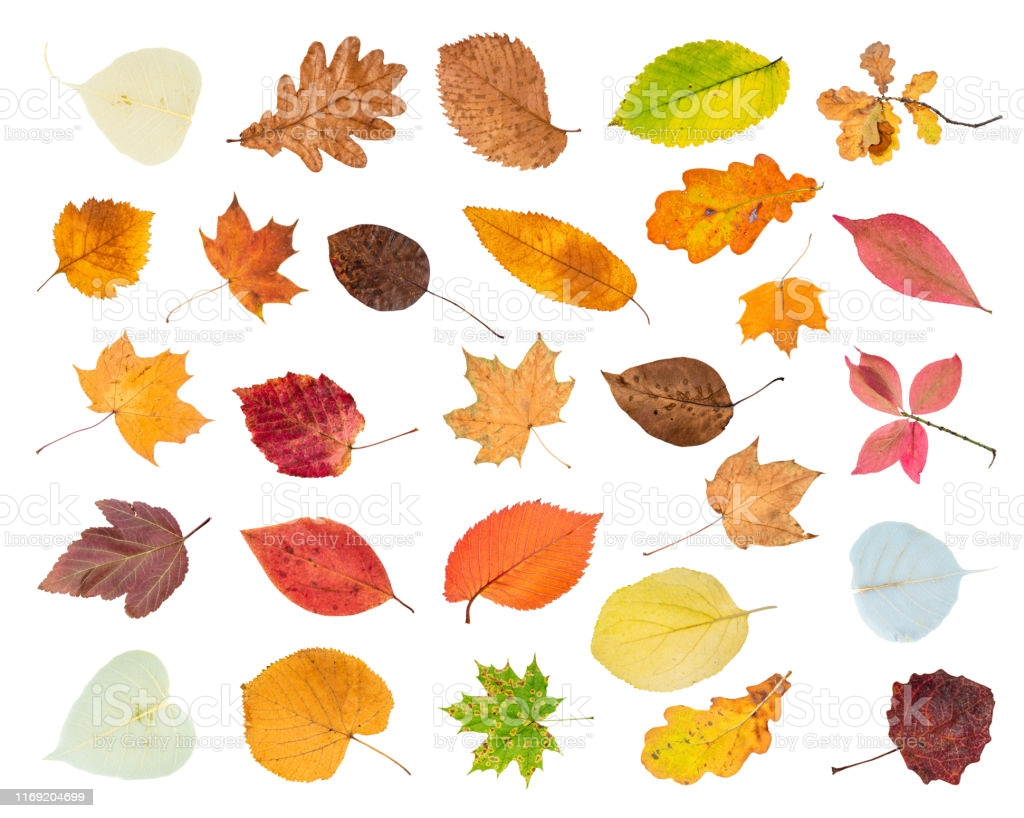
\includegraphics[width=7cm]{img.jpg}\label{fig:a}}\hspace*{3em}%
 \subfloat[inscribed circles (color inverted)]{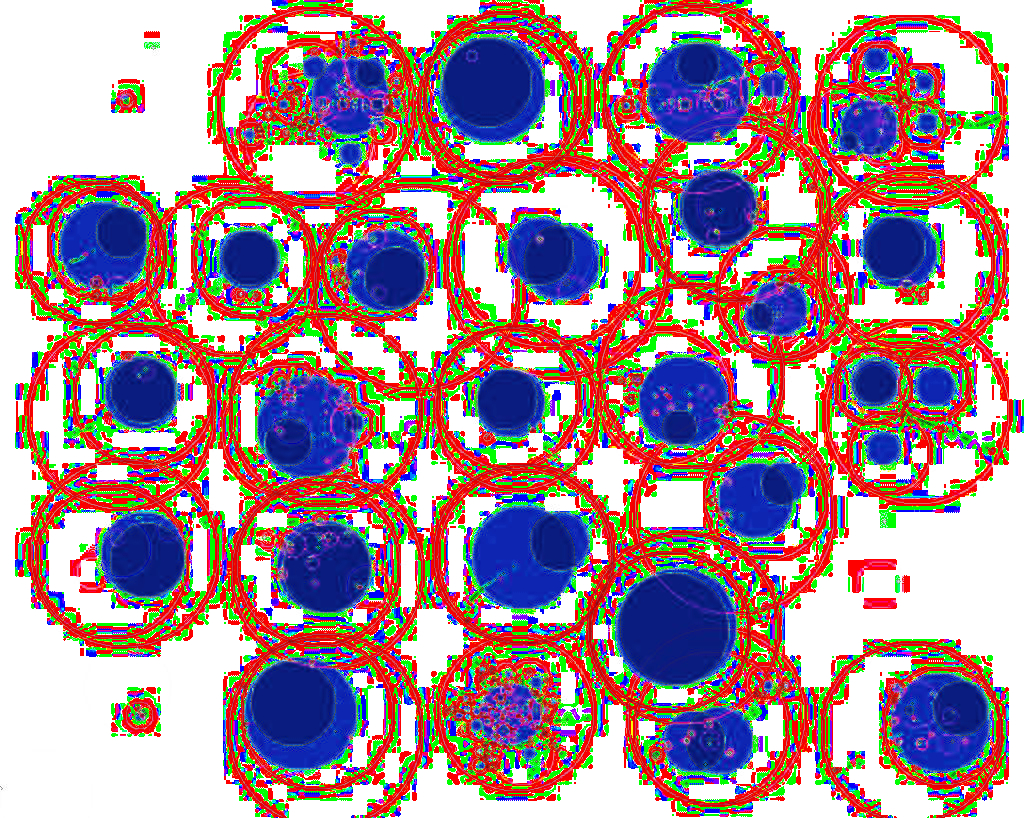
\includegraphics[width=7cm]{i2a.jpg}\label{fig:b}}\\
 \subfloat[filtered contours (color inverted)]{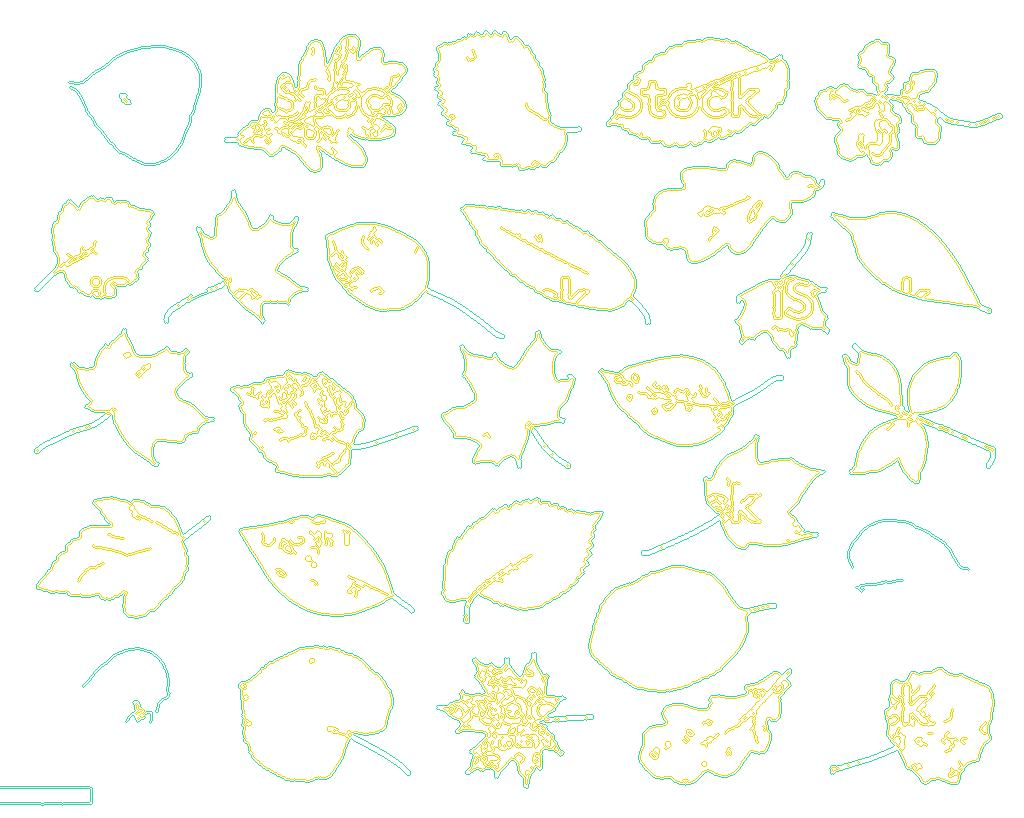
\includegraphics[width=7cm]{i1a.jpg}\label{fig:c}}\hspace*{3em}%
 \subfloat[insribed circles (enlarged)]{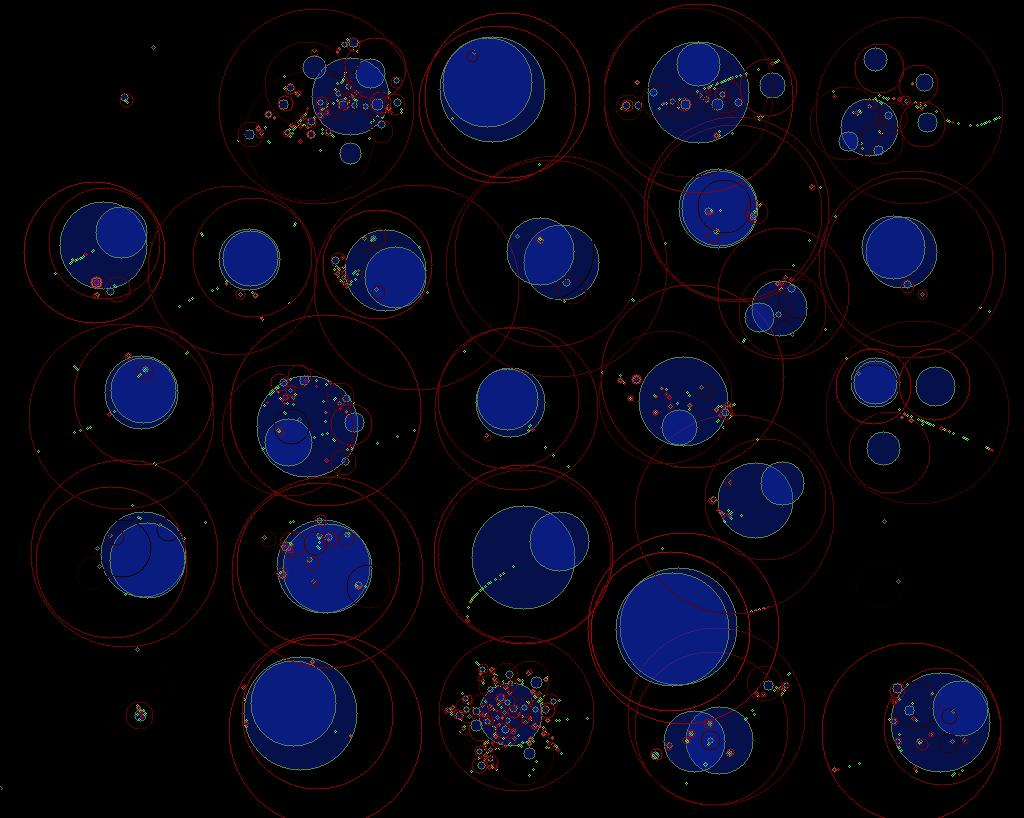
\includegraphics[width=7cm, trim=
    4cm 4cm 4cm 1cm, clip]{i2.jpg}\label{fig:d}}\\
 \subfloat[convex hull with bounding rectangles]{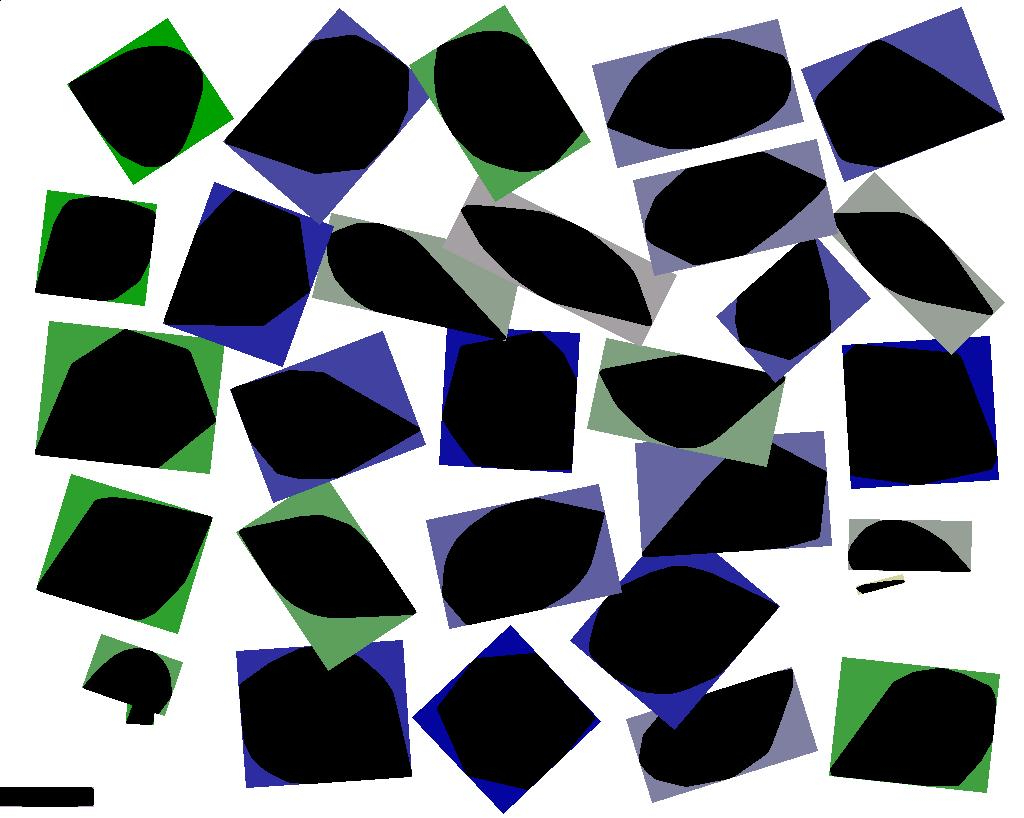
\includegraphics[width=7cm]{i3a.jpg}\label{fig:e}}\hspace*{3em}%
 \subfloat[interior-contour color average]{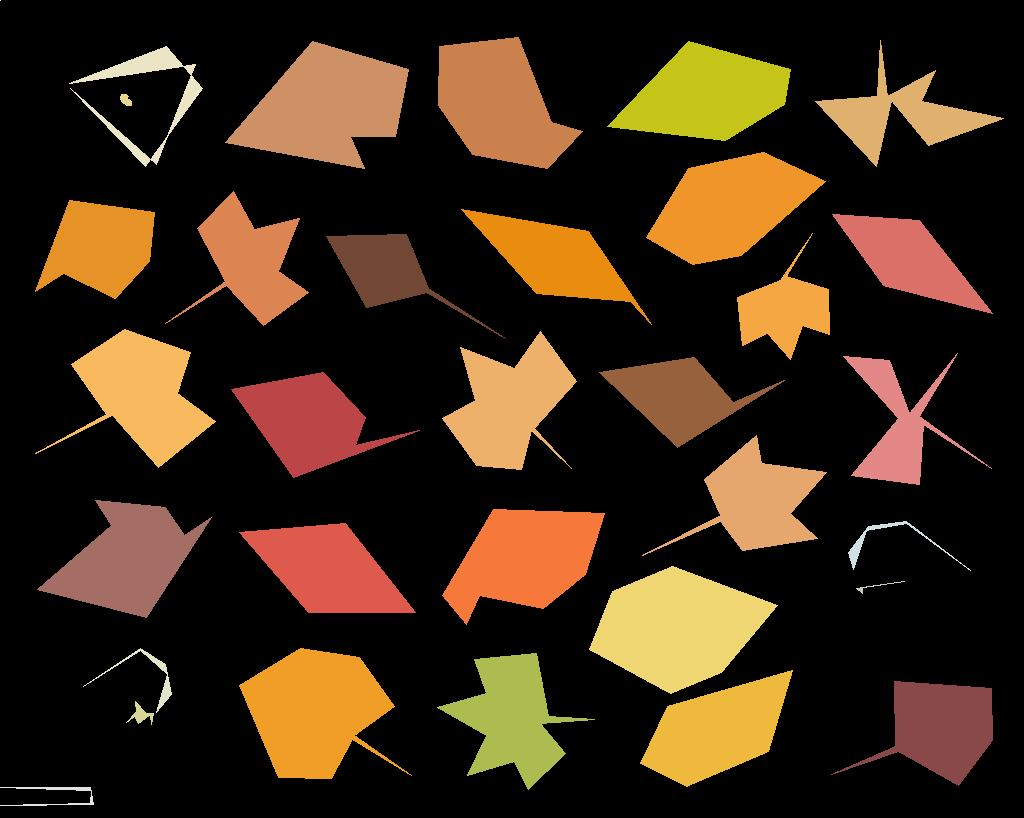
\includegraphics[width=7cm]{i4.jpg}\label{fig:f}}\\
 \caption{Visualizing Contour Feature-Vectors}%
 \label{fig:all}%
(note that in (e) the colors are inverted, and the gap 
between the convex hull and bounding rectangle is shaded to 
visualize the angle of the rectangle to external image borders)
\vspace{2em}
\end{figure*}


\p{All of these metrics classify regions only on basic 
mathematical levels; none of this quantitative 
data suffices to discern whether contour-delimited 
regions correspond to cells, cars, or any other kind of 
real-world objects.  Nevertheless, region feature-vectors 
are the starting point for statistical calculations 
which lead to more sophisticated image-tagging.  This 
is roughly a two-step process, first identifying regions which 
seem likely to correspond to real-world objects and then 
classifying those objects themselves.  In the biomedical 
context, image-tagging involves classifying regions 
which are biologically and/or diagnostically significant.  
An image-processing algorithm might attempt to isolate a solid-tumor 
mass, for example; such an algorithm may be able to correctly 
demarcate the region of an image where a tumor is visible.  
For diagnostic purposes further details would then need to 
be added, classifying tumors into categories such as 
\q{sarcomas larger than 5cm.}  Such classifications 
may or may not be possible with automated tools; 
traditionally these details are added by radiologists 
or pathologists who manually examine radiographic 
images, although image-analysis tools could be used 
to expedite this process (e.g., to select the 
most diagnostically valuable images from a \DICOM{} 
image-series).}

\p{The end result of biomedical image-analysis is of 
course these diagnostic or investigative annotations, such as 
labeling an image-region as a particular kind of tumor, 
with a particular size and characteristics --- these are the 
details generally recorded in an annotated imaging database 
or notated via \DICOM{} extensions such as Treatment Plans 
or Structured Reports.  Data of a more quantitative sort, such 
as the feature-vectors characterizing image contours, is 
important only as an intermediary processing step.  Nevertheless, 
there are several reasons why intermediate image-analysis data 
may continue to be important even after the higher-level and 
more \q{semantic} (as opposed to purely quantitative) analytic 
steps have occurred.}

\p{For one thing, it is inconvenient 
for pathologists/radiologists to manually mark off image regions in the course 
of reporting their diagnostic findings.  As such, 
machine-segmented Regions of Interest (or some subspace derived 
from them, such as a polygonal frame enclosing their convex hull) 
can be integrated into diagnostic reports, which means that 
techniques must be applied to incorporate mathematically extracted 
contours/regions into image annotations.  Moreover, 
there are scenarios where behind-the-scenes image process 
data may need to be retained for subsequent research; this data 
may be relevant for holistic statistical analysis of 
large-scale data-sets and/or for revisiting diagnoses over time.  
For instance, a software component may try to measure the progression 
of a tumor by comparing automatically-extracted image regions 
taken at two different times, assuming that the corresponding 
regions depicting \q{the same} tumor can be isolated 
and then mathematically compared.}

\p{For these kinds of scenarios, it is reasonable to assume that 
at least some intermediate image-processing data should be 
retained for subsequent analysis, which then raises the 
question of how image-feature vectors should optimally be 
represented in a database context.  We will address this question 
in a later chapter.}

\p{Similar comments apply also 
to audio feature-vectors, such as those derived from 
Fast Fourier Transforms (\FFT{}) or  
Mel-Frequency Cepstral Coefficients (\MFCC{}), 
which in bioinformatics may classify \EKG{}s, 
sonograms, and other biologically useful audio resources; 
\cite{AuroreLyon} summarize that for 
EKG{} signals \q{[m]orphological features include the coefficients of the 
Hermite transform, the wavelet transform or the discrete cosine transform 
... that aim to model the ECG beat instead of 
extracting features from the raw data} (page 2).
Because machine-learning and other statistical analytic techniques operate 
on \EKG{} feature vectors, these vectors serve 
as intermediate representations of \EKG{} waveforms from which diagnostic 
findings are derived.  The process of extracting feature-vectors 
from audio waveforms bears some mathematical similarities 
to that of extracting feature-vectors from Distinguished Regions 
of bioimages (reflected in the extension of \DICOM{} to 
encompass audio assets), which will be emphasized in later chapters.}

\subsection{Common Data Models for Clinical Research}

\p{Other biomedically important data structures derive from initiatives to 
share or pool clinical data for research purposes.  A good example of 
such an initiative is the \OMOP{} partnership mentioned 
earlier.  The \OMOP{} format prioritizes data-integration 
according to largely conventional \SQL{} paradigms; in 
the \OMOP{} context most information is held in relational 
databases, and data integration involves merging disparate 
database tables.  Toward that end, the Common Data Model 
standardizes those specific tables which should be present 
among compliant data sets and the columns within each of 
these tables, where the various columns are given a 
canonical name and data type.  For example, specific tables 
include ones for personal (patient) information, 
data about a specific visit made by a patient to a health-care
provider, data about one specific procedure administered to a 
patient, information about a specific occasion when a patient 
received a drug/pharmaceutical, data about the costs of either 
drugs or procedures (or other \q{medical events}), and so forth.  
The point is not that health care providers' software would 
internally store information with this precise configuration 
of tables, but rather that biomedical data (in whatever format 
internally used) can be shared by distributing each data field 
into the specific collection of tables and columns 
mandated by the \OMOP{} \CDM{}.  The key data-integration step in 
this case is then whichever algorithms each individual institution 
uses to initialize \OMOP{} tables from local information.}

\p{Readers who would like to examine the specific tables and columns 
which constitute the \OMOP{} Common Data Model may consult the 
source code accompanying this book (see the \textbf{omop} project).  
This code implements \Cpp{} classes corresponding to \OMOP{} \CDM{} 
tables.  The project is not an \OMOP{} client as such 
--- there is no logic for populating the tables from a database 
instance --- but it serves as a reference illustrating the 
fields and structures which are endemic to \OMOP{} data representations.} 

\p{The accompanying code similarly has a \textbf{pcor} project 
which demonstrates the \PCORnet{} Common Data Model.  Similar to 
the \OMOP{} \CDM{}, this standard (developed by the 
National Patient-Centered Clinical Research Initiative) 
promotes data integration by specifying that 
shared data be distributed into a collection of tables 
with fixed roles and column-sets.  The various tables include 
a \q{Demographic} specification with essential personal 
patient info, a table representing patients' enrollment 
in a clinical trial, a \q{Dispensing} table noting medicines 
dispensed by a pharmacy to a patient, and tables for diagnoses, 
lab results, \q{vital signs,} and so forth.  It is interesting 
to contrast the \OMOP{} and \PCORnet{} Common Data Models, 
which can be readily compared because they are structurally similar; 
the fact that they nonetheless recognize fairly different table and column 
sets point to the specific interests of Observational Medicine 
and of patient-centered advocacy, respectively.}

\p{In contrast to the table-based and \SQL{}-inspired formats 
for \OMOP{} and \PCORnet{}, parts of the \CDISC{} standard 
lean more toward Semantic Web information structures 
(as with the \BRIDG{} --- Biomedical Research Integrated 
Domain Group --- specification which is one of several \CDISC{} 
standard models).  The contrast between table-oriented 
and Semantic Web notions of a \q{controlled vocabulary} 
embody alternative theories of the role of semantic normalization 
in technology.  For table-oriented environments, Controlled 
Vocabularies specifically address the organization of 
digital resources; for example, table names, column names, 
and in some cases the values asserted within columns are 
required to have identifiers drawn from a restricted 
class of terms.  This restriction applies to 
individual values when those values are neither numeric nor 
string types (such as a person's name, which for obvious reasons 
cannot be tied to a list of accepted values) but rather to 
columns whose data may reasonably restricted to a given 
enumeration.  For instance, the state where a patient 
resides must be one of the fifty US states (assuming a patient is 
an American citizen and excluding, for sake of argument, 
territories such as the District of Columbia).  It is possible 
to write or abbreviate state names in different ways, but 
a Controlled Vocabulary could reasonably stipulate that all 
conformant data sets use identical terms 
for the same state name.}

\p{This discussion uses terminology associated with 
relational database tables; for general discussion 
of data-integration it makes sense however to 
adopt more type-theoretic language, so that 
we can consider the names of data types, the names 
of the fields which data types contain, and 
(in some cases) the values which are spanned by 
those fields.  In lieu of restricting names to 
data types themselves, a system may instead assign 
names to \textit{interfaces}, or in effect to 
prototypes and specifications which data types need 
to put into operation.  A protocol may specify a 
collection of interfaces, and a software component 
which implements the protocol will provide one data 
data for each interface that the protocol outlines.  
Controlled Vocabularies therefore specifies the names 
of interfaces, as well as the names of data fields 
accessed through the values which instantiate data 
types implementing each interface.  Controlled Vocabularies 
would also specify the range of nominal values assigned 
to enumerative types, in the case of data types whose 
values derive from a specified list (e.g., the set of 
US states).
}

\p{In the case of Semantic Web data, by contrast, Controlled 
Vocabularies (typically called \q{Ontologies} in this 
context) serve a more generic role, typically connecting 
data types not only to particular software implementations 
but also to more abstract concepts.  For example, cancer 
is classified (according to histological criteria) 
into one of six groups (Carcinoma, Sarcoma, Myeloma, 
Leukemia, Lymphoma and Mixed).  A data-representation 
standard could reasonably stipulate that any tumor 
--- that is, any data structure describing the characteristics 
of a tumor --- include a data field classifying the 
tumor into one of the six groups (at least those whose 
cancers present as tumors that can be detected via bioimaging).  
In this sense the six groups (and canonical names associated 
with them) constrain the range of values spanned by a 
cancer-type (and by extension tumor-type) data field.  
Such a formal stipulation can be defined both as a restriction 
on table data and as part of a Semantic Web Ontology; in short, 
semantic standardization at this level is common to both 
paradigms.  However, an Ontology may further model 
\q{philosophical} traits associated with a tumor; for instance, 
the fact that a tumor is a form of biological tissue, and 
more generally a biological entity, which in turn 
is a physical thing, possessing characteristics such as size and 
volume.  These more general concepts do not fit 
within type systems themselves --- there is rarely a 
data type modeling \q{physical things} in general --- so 
the purpose of Standardized Vocabularies in contexts 
such as the Semantic Web is not merely to 
serve as a guideline for implementing 
code libraries (e.g., those that would export data 
in the \OMOP{} or \PCORnet{} Common Data Models) 
but as a basis for Artificial Intelligence.  In this sense 
the values which are represented within Semantic Web 
data structures may in some cases be associated with 
specific computational data types, but they are 
also modeled in terms of networks of concepts 
that are designed to serve as a foundation for \AI{} 
reasoning.}

\p{Later in the book we will return to the 
role of Ontologies and other meta-models in 
data-integration contexts.  Before engaging 
these more theoretical discussions, however, we 
will try to develop a more substantial 
concrete picture of how data-integration problems 
arise.  This discussion will be the focus of the 
following chapter, beginning with further consideration 
of the overlap between data-integration challenges 
and Precision Medicine.}


%\section{}

%using a data-integration framework that captures the full heterogeneity 
%of patient health data which would include everything from biochemical 
%assays to image studies.  \footnote{LTS's tools are in very much in keeping 
%with precision medicine guidelines.  Such guidelines are 
%elucidated by Shrestha and his coauthors elucidate 
%these guidelines 
 
%who  

